\chapter{Implementace}

% TODO: napsat úvod kapitoly (přehled, co bude v této kapitole)

\section{Specifikace pravidel požadovaných zadáním práce}
Nejprve definujeme vhodný predikát, který nám umožní vybrat množiny vrcholů tak, abychom mohli specifikova LoD. Vybrané množiny potom ověříme pomocí predikátu, který určí, zda jsou tyto množiny v~pořádku, či zda porušují \emph{LoD} princip.

\begin{definition}
Mějme grafový model projektu $G = \langle V, E, \rho, K, C, N, \mathit{Kind}, \mathit{Classifier}, \mathit{Name}\rangle$. Definujme selektor vrcholů $F(G, v', k', c')$, $v' \in V$, $k' \in K$, $c' \in C$ jako množinu vrcholů $v \in V, Kind(v) = k'$, které jsou dostupné z~vrcholu $v'$ pomocí orientované cesty, pro jejíž všechny vrcholy $v''$ s~výjimkou posledního platí $Kind(v'') \ne k'$ a která obsahuje hranu $e$, pro niž platí $Classifier(e) = c' $.
\end{definition}

\subsection{Law of Demeter}
\label{implementation-lod_specification}
Pro definici princip LoD si zavedeme speciální typ grafového modelu. Ačkoliv jsme pojem \emph{typ grafového modelu}  přesně nedefinovali a zavedli jej pouze intuitivně, pokusíme se nyní vymezit pojem \emph{demeter graph model}, který zde budeme dále používat, přesněji.

U grafového modelu typu \emph{Demeter graph type} povolíme libovolná označení vrcholů (konkrétně pro potřeby LoD se bude jednat o plně kvalifikované názvy tříd a metod). Množinu typů vrcholů omezíme na následující množinu:
\begin{align*}
K = \{ ``class", ``method" \}
\end{align*}
Význam těchto typů je zřejmý. Typ \emph{class} použijeme pro vrcholy, které budou odpovídat deklarovaným třídám v existujícím projektu a typ \emph{method} bude označovat jejich metody.

Taktéž množina klasifikátorů hran nebude libovolná, ale bude přesně daná:
\begin{align*}
C = \{ ``field", ``self", ``arg", ``constr", ``use" \}
\end{align*}
Podívejme se na význam těchto označení:
\begin{itemize}
\item $``field"$ -- hrana vede do třídy, které reprezentuje třídní promenou nebo do její nadtřídy
\item $``self"$ -- hrana vede do třídy, která je vlastníkem této metody nebo do její nadtřídy
\item $``arg"$ -- hrana vede do třídy argumentu metody nebo do její nadtřídy
\item $``constr"$ -- hrana vede do třídy použité pro konstrukci nového objektu v těle metody nebo do její nadtřídy
\item $``use"$ -- hrana vede do třídy, jejíž použití (vyvolání metody nebo přístup k poli) se vyskytuje v těle metody
\end{itemize}
Je patrné, že tyto hrany zčásti odpovídají požadavkům LoD. Prozatím jsme uvedli množiny klasifikátorů bez vymezení, kde lze přesně tyto klasifikátory použít. Uvažujme následující množinu, která reprezentuje zobrazení množiny klasifiktároů do množiny dvojic typů vrcholů:
\begin{align*}
GT = &\{ \\
&(``field" (``class", ``class")), \\
&(``self" (``method", ``class")), \\
&(``arg" (``method", ``class")), \\
&(``use" (``method", ``class")), \\
&(``use" (``method", ``class")) \\
&\}
\end{align*}
Pokud budeme uvažovat koncové vrcholy jednotlivých hran a jejich zobrazení do množiny typů, potom musí platit, že obraz jednotlivých komponent hrany (vrcholů) bude shodný s~obrazem hrany provedeného pomocí zobrazení GT.

Pokud \emph{grafový model projektu splní} všechny tyto podmínky, řekneme o něm, že je typu \emph{demeter graph model}.

Příklad takového grafu je na obrázku \ref{implementation-lod_graph}. Lze jej získat ze zdrojových kódů pogramu.

% TODO: aktualizovat graf!!!
\begin{figure}[h!]
  \centering
  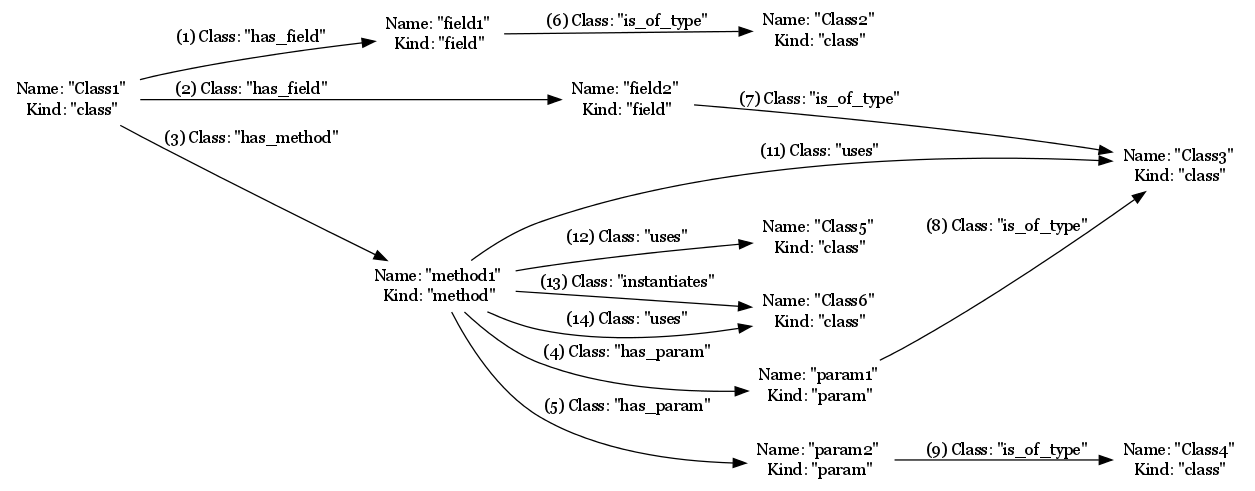
\includegraphics[width=1.0\textwidth]{./graphs/demeter_graph.png}
  \caption{Graf použitý pro validaci principu LoD.\label{implementation-lod_graph}}
\end{figure}

Pravidlo LoD potom specifikujeme následovně:

\begin{designprinciple}
Mějme grafový model projektu $G = \langle V, E, \rho, K, C, \mathit{Kind}, \mathit{Classifier}\rangle$. Návrhový princip LoD splňuje graf, pro který platí:

\begin{align*}
\forall v \in V: Kind(v) = ``method"\\
\end{align*}
\begin{align*}
&F(v, ``method", ``use") \setminus ( F(v, ``method", ``self") \cup F(v, ``method", ``field") \cup \\
&F(v, ``method", ``arg") \cup F(v, ``method", ``constr")) = \emptyset
\end{align*}

\end{designprinciple}

% TODO: opravit!
Specifikované pravidlo vyjadřuje požadavek, aby množina vrcholů do níž se dostaneme pomocí hran, které představují povolené vstupy tříd do analyzované třídy (třídní proměnné, parametry, vytvářené objekty), byla totožná s~množinou všech vrcholů, které představují všechny třídy používané (klasifikátor $``uses"$) v~rámci některé z~metod. Odečtení vrcholu $v$ z~výsledné množiny je zde kvůli tomu, abychom nemuseli navíc zavádět zbytečnou hranu identifikující, že třída je známá sama sobě.

\subsection{Low coupling, high cohesion}
% TODO:
% odkázat na rešeši v analýze a přidat poznámku o tom, že tato pravidla nebyla specifikována s tím, že je možné je realizovat jako analýzu pomocí rozhraní AnalysisIface

\section{Implementace jádra systému}
% TODO: incorporate
Implementujeme jako netbeans modul av-core

\subsection{Implementace formátu AVD}
%% TODO: sort and formulate
ValidationModel v~sobě bude zapouzdřovat data z~AVD souborů. AVD soubory budou mít samostatné jmenné prostory pro následující typy jmen:

\begin{itemize}
\item názvy analýz
\item jména typů grafů
\item jména atomických a složených pravidel (jmenný prostor pro atomická i složená pravidla je sdílený)
\item jména operátorů
\item datové typy v modelu
\end{itemize}

\begin{itemize}
\item AVD formát
\item definice gramatiky
\end{itemize}

\subsection{Implementace sestavování validačního modelu}
\begin{itemize}
\item ANTLR -- vybudování ast
\item postupné sestavování vyhodnocovacího stromu
\end{itemize}

\subsection{Implementace základních operátorů}
Vyhodnocení univerzálního kvantifikátoru $\forall v \in V$ lze přepsat jako jednoduchý cyklus přes vrcholy vrácené zpřesňující operátorem, která vybírá nějakou podmnožinu z~množiny vrcholů analyzovaného grafu. Získáme tak kód podobný listingu \ref{listing-forall}. V~tomto kódu, který je fragmentem metody, používáme symoblický název \verb+condition+ pro podmínku, kterou musí splňovat každý prvek \emph{v} iterované kolekce vrcholů \emph{vertices}.

\begin{lstlisting}[
    language=java,
    caption={Implementace univerzálního kvantifikátoru $\forall$.},
    label=listing-forall
  ]
for (Vertex v : vertices) {
    if (!condition(v, ...)) {
        return false;
    }
}
return true;
\end{lstlisting}

Analogicky budeme postupovat u~existenčního kvantifikátoru $\exists$. Zde nám stačí nalézt alespoň jeden element, pro který vyhodnocovaná vlastnost platí. Listing \ref{listing-exists} představuje fragment metody. Pokud se podaří nalézt alespoň jeden prvek, který splňuje požadovanou podmínku, metoda vrátí hodnotu \emph{true}. Vzhledem k~použití příkazu \emph{return} je zřejmé, že dochází k~\uv{línemu} vyhodnocování -- vyhodnocení je ukončeno nalezením prvního vyhovujícího elementu (další se neprohledávají). Stejně jako u~operátoru $\forall$ i zde název \verb+condition+ symbolizuje konkrétní podmínku, která má platit nad alespoň jedním prvkem množiny uzlů.

\begin{lstlisting}[
    language=java,
    caption={Implementace existenčního kvantifikátoru $\exists$.},
    label=listing-exists
  ]
for (Vertex v : vertices) {
    if (condition(v, ...)) {
        return true;
    }
}
return false;
\end{lstlisting}

Můžeme si všimnout, že se obě implementace liší pouze přehozením podmínek -- zatímco v~prvním případě ($\forall$) musíme projít všechny prvky, abychom zjistili, zda všechny prvky splňují požadovanou vlastnost, ve druhém případě ($\exists$) budeme všechny prvky procházet pouze v~krajním případě, kdy vlastnost neplatí pro žádný z~prvků.

\section{Implementace modulů rozšíření}

% TODO: rozepsat
\begin{itemize}
\item SPI -- implementace rozhraní
\item pojem \emph{poskytovatel služby}
\item lookup, META-INF/services, registrace služeb
\end{itemize}

\subsection{Modul av-graphgen-demeter (generátor grafu)}
ukázkový poskytovatel generátoru grafu

Implementujeme jako samostatný netbeans modul.

\emph{DemeterGraphGenerator} implementuje \emph{GraphGeneratorIface}.

Zpracovávání AST:
Vyhledávali jsme:
\begin{itemize}
\item visitClass
\item visitMethod
\item visitVariable
\item visitIdentifier
\item visitMethodInvocation
\item visitMemberSelect
\item visitNewClass
\item visitNewArray
\end{itemize}

\begin{itemize}
\item použití zásobníku
\item generování hran
\end{itemize}

\begin{itemize}
\item ``field" -- visitVariable, visitIdentifier
\item ``self" -- enclosing element
\item ``arg" -- visitVariable (level 3)
\item ``constr" -- new, new array
\item ``use" -- method invocation, member select (přístup k polím třídy)
\end{itemize}

\subsection{Modul av-operators-demeter (operátory pro LoD)}
ukázkový balíček operátorů pro ověřování principu LoD

\begin{itemize}
\item třída \emph{EmptyVertexSetPredicate} -- \uv{empty} -- $P() = \emptyset$
\item třída \emph{FVertexSetSelector} -- \uv{F} -- popsáno výše
\item třída \emph{VertexKindPredicate} -- \uv{kind} -- $Kind(v, ``label")$
\end{itemize}

Obsahuje sadu tříd implementující operátory potřebné pro definování pravidla pro validaci LoD. Tyto třídy implementují rozhraní \emph{OperatorIface} (resp. jeho podtypy).

\section{Integrace do NetBeans IDE}

%% TODO: incorporate
%% (modul av-platform-integration)

Při implementaci bylo hojně využíváno informací z~\cite{netbeans_platform}.

% TODO: write about actions, about usage of the ArchVal API
Seznam integračních komponent je k~dispozici v~tabulce \ref{implementation-integration_components}.

% TODO: zkontrolovat tabulku integračních komponent
\begin{table}
  \caption{Tabulka integračních komponent systému. \label{implementation-integration_components}}
  \begin{center}
    \begin{tabular}{ | l | l | p{8cm} | }
      \hline
      \textbf{Název} & \textbf{Typ} & \textbf{Zodpovědnost} \\
      \hline
      \hline
      ValidateMainProject & class & integrace s~běhovou platformou, vstupní/aktivační bod \\ \hline
      %% TODO: 'třída implementující rozhraní...'
      GraphGeneratorRegister & class & třída poskytující přístup k~informacím o~existujících poskytovatelích generátorů grafu \\ \hline
      OperatorRegister & class & třída poskytující přístup k~informacím o~existujících poskytovatelích operátorů \\ \hline
      AnalysesRegister & class & třída poskytující přístup k~informacím o~existujících poskytovatelích komponent analýzy \\ \hline
    \end{tabular}
  \end{center}
\end{table}

\subsection{Použití jádra systému ArchVal}
% TODO: rozepsat
Zabalení třídy ArchVal do singletonu ArchvalInstance

\subsection{Přidání uživatelské akce do nabídky prostředí}
Třída \emph{ValidateMainProject}

Integrace do běhové platformy. Reprezentuje uživatelskou akci. Bude implementováno na základě zvolené implementační platformy (akce v~GUI).

\subsection{Vstupní rozhraní}
% TODO: reorder to fit right order
\subsubsection{Ukázka vstupního formátu}
\lstinputlisting[
  label=avdgrammar,
  caption={Ukázka vstupního AVD souboru odpovídajícího pravidlu specifikovanému v podsekci \ref{implementation-lod_specification} (LoD).}
]{./listings/example.avd}

\subsection{Výstupní rozhraní}
% TODO: zde popsat implementované výstupní rozhraní (alternativy by měly být diskutovány v návrhu)
% TODO: textový výstup

\subsection{Implementace registrů poskytovatelů služeb}
% TODO: rozepsat, přidat ukázku kódu
\begin{itemize}
\item SPI
\item NetBeans lookup -- /META-INF/services
\end{itemize}

\subsubsection{Podpora editace AVD souborů}
% TODO: rozepsat
\begin{itemize}
\item experimentální mime typ \verb+text/x-avd+
\item třída \emph{AvdCookie}
\item zvýrazňování syntaxe (modul av-avd-highlighter)
\end{itemize}
